%sf bay is screwed
We focus on the San Francisco Bay Area, a seismically-active region with a complex web of roads and transit networks, to illustrate our approach (Figure~\ref{fig:equity_study_area}). The area follows a polycentric metropolitan form, with San Francisco as the primary center and other jobs  concentrated in suburban centers, such as Silicon Valley~\cite{cervero_polycentrism_1997}. The region has a wide array of trip patterns for mandatory and non-mandatory trips. Furthermore, trip times and routes vary greatly depending on travel preferences and workplace locations~\cite{cervero_polycentrism_1997}. Thus,  we might expect noticeable disparities between households in the risk of travel time delays due to earthquakes. 


%and here are the study area and models
As described in Section~\ref{sec:caseMet}, we consider the road network and the relevant transit systems. We  model damage to bridges and other structures from a probabilistic set of earthquake events in order to predict the loss in mode-destination accessibility (as introduced in Section~\ref{sec:accessibility}).
%no surprises
From a large set of ground-motion intensity maps and damage maps, we choose a set of forty maps, using the optimization procedure presented in Chapter~\ref{chapt:opt}; we chose the fixed-demand travel time delay as the proxy metric, because it is related to travel time delays expected in the high-fidelity model. We then use the high-fidelity model to predict the transportation network impacts of the forty pairs of ground-motion intensity and damage maps. Readers are referred to Appendix~\ref{chapt:b} for a step-by-step procedure for aggregating the requisite data sources, modeling interdependencies, and adapting an activity-based transportation model for catastrophe risk assessment. The outcome is forty sets of results for the target performance metric, mode-destination accessibility (Section~\ref{sec:accessibility}). Each accessibility value has a corresponding annual rate of occurrence.
In the following sections, we first compare region-wide results, and then focus on particular characteristics of three communities (Figure~\ref{fig:equity_study_area} shows the study area and three communities). Finally, we discuss generalizable trends.
\begin{figure}
\centering
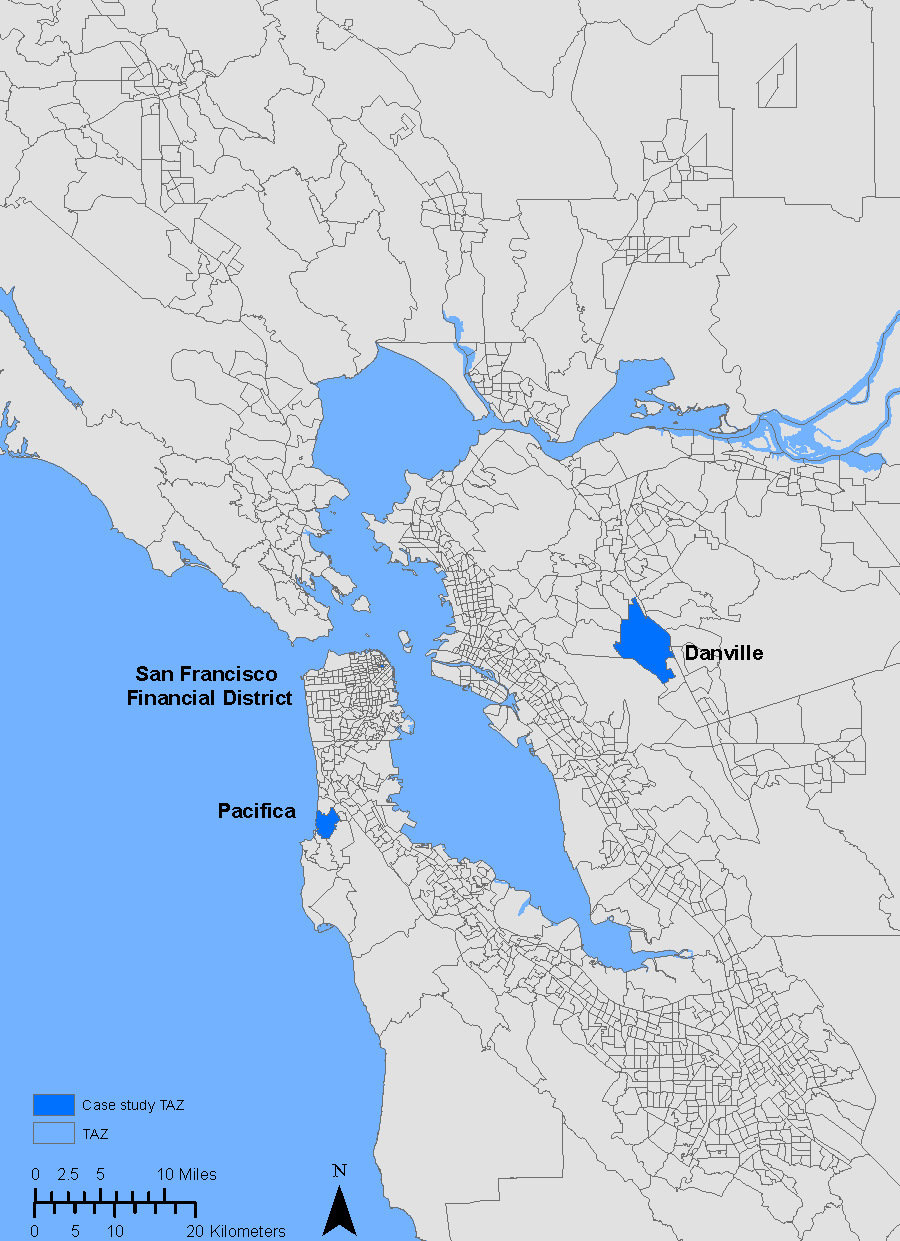
\includegraphics[width=6in]{FIGS/equity_case.pdf} 
\caption{Study area: San Francisco Bay Area, CA with specific travel analysis zones (TAZs) used in the case study marked in blue.}
\label{fig:equity_study_area}
\end{figure}

